%%% Local Variables:
%%% mode: latex
%%% TeX-master: ".."
%%% End:

\documentclass[border=5]{standalone}
\usepackage[svgnames]{xcolor}
\usepackage[T1]{fontenc}
\usepackage{xeCJK}
\usepackage{tikz}
\usetikzlibrary{arrows,decorations.pathmorphing,backgrounds,
positioning,fit,shapes.misc,calc}

\tikzset{line/.style={
         color=#1,line width=5pt,line join=round,inner sep=0pt}}
\tikzset{stop/.style={
         draw,color=#1,shape=circle,very thick,fill=white,minimum width=0.4cm,inner sep=0pt}}
\tikzset{stop-terminal/.style={
         draw,color=#1,shape=circle,fill=#1,minimum width=0.5cm,inner sep=0pt}}

\pgfdeclarelayer{line}
\pgfdeclarelayer{stop}
\pgfsetlayers{line,stop}

\begin{document}
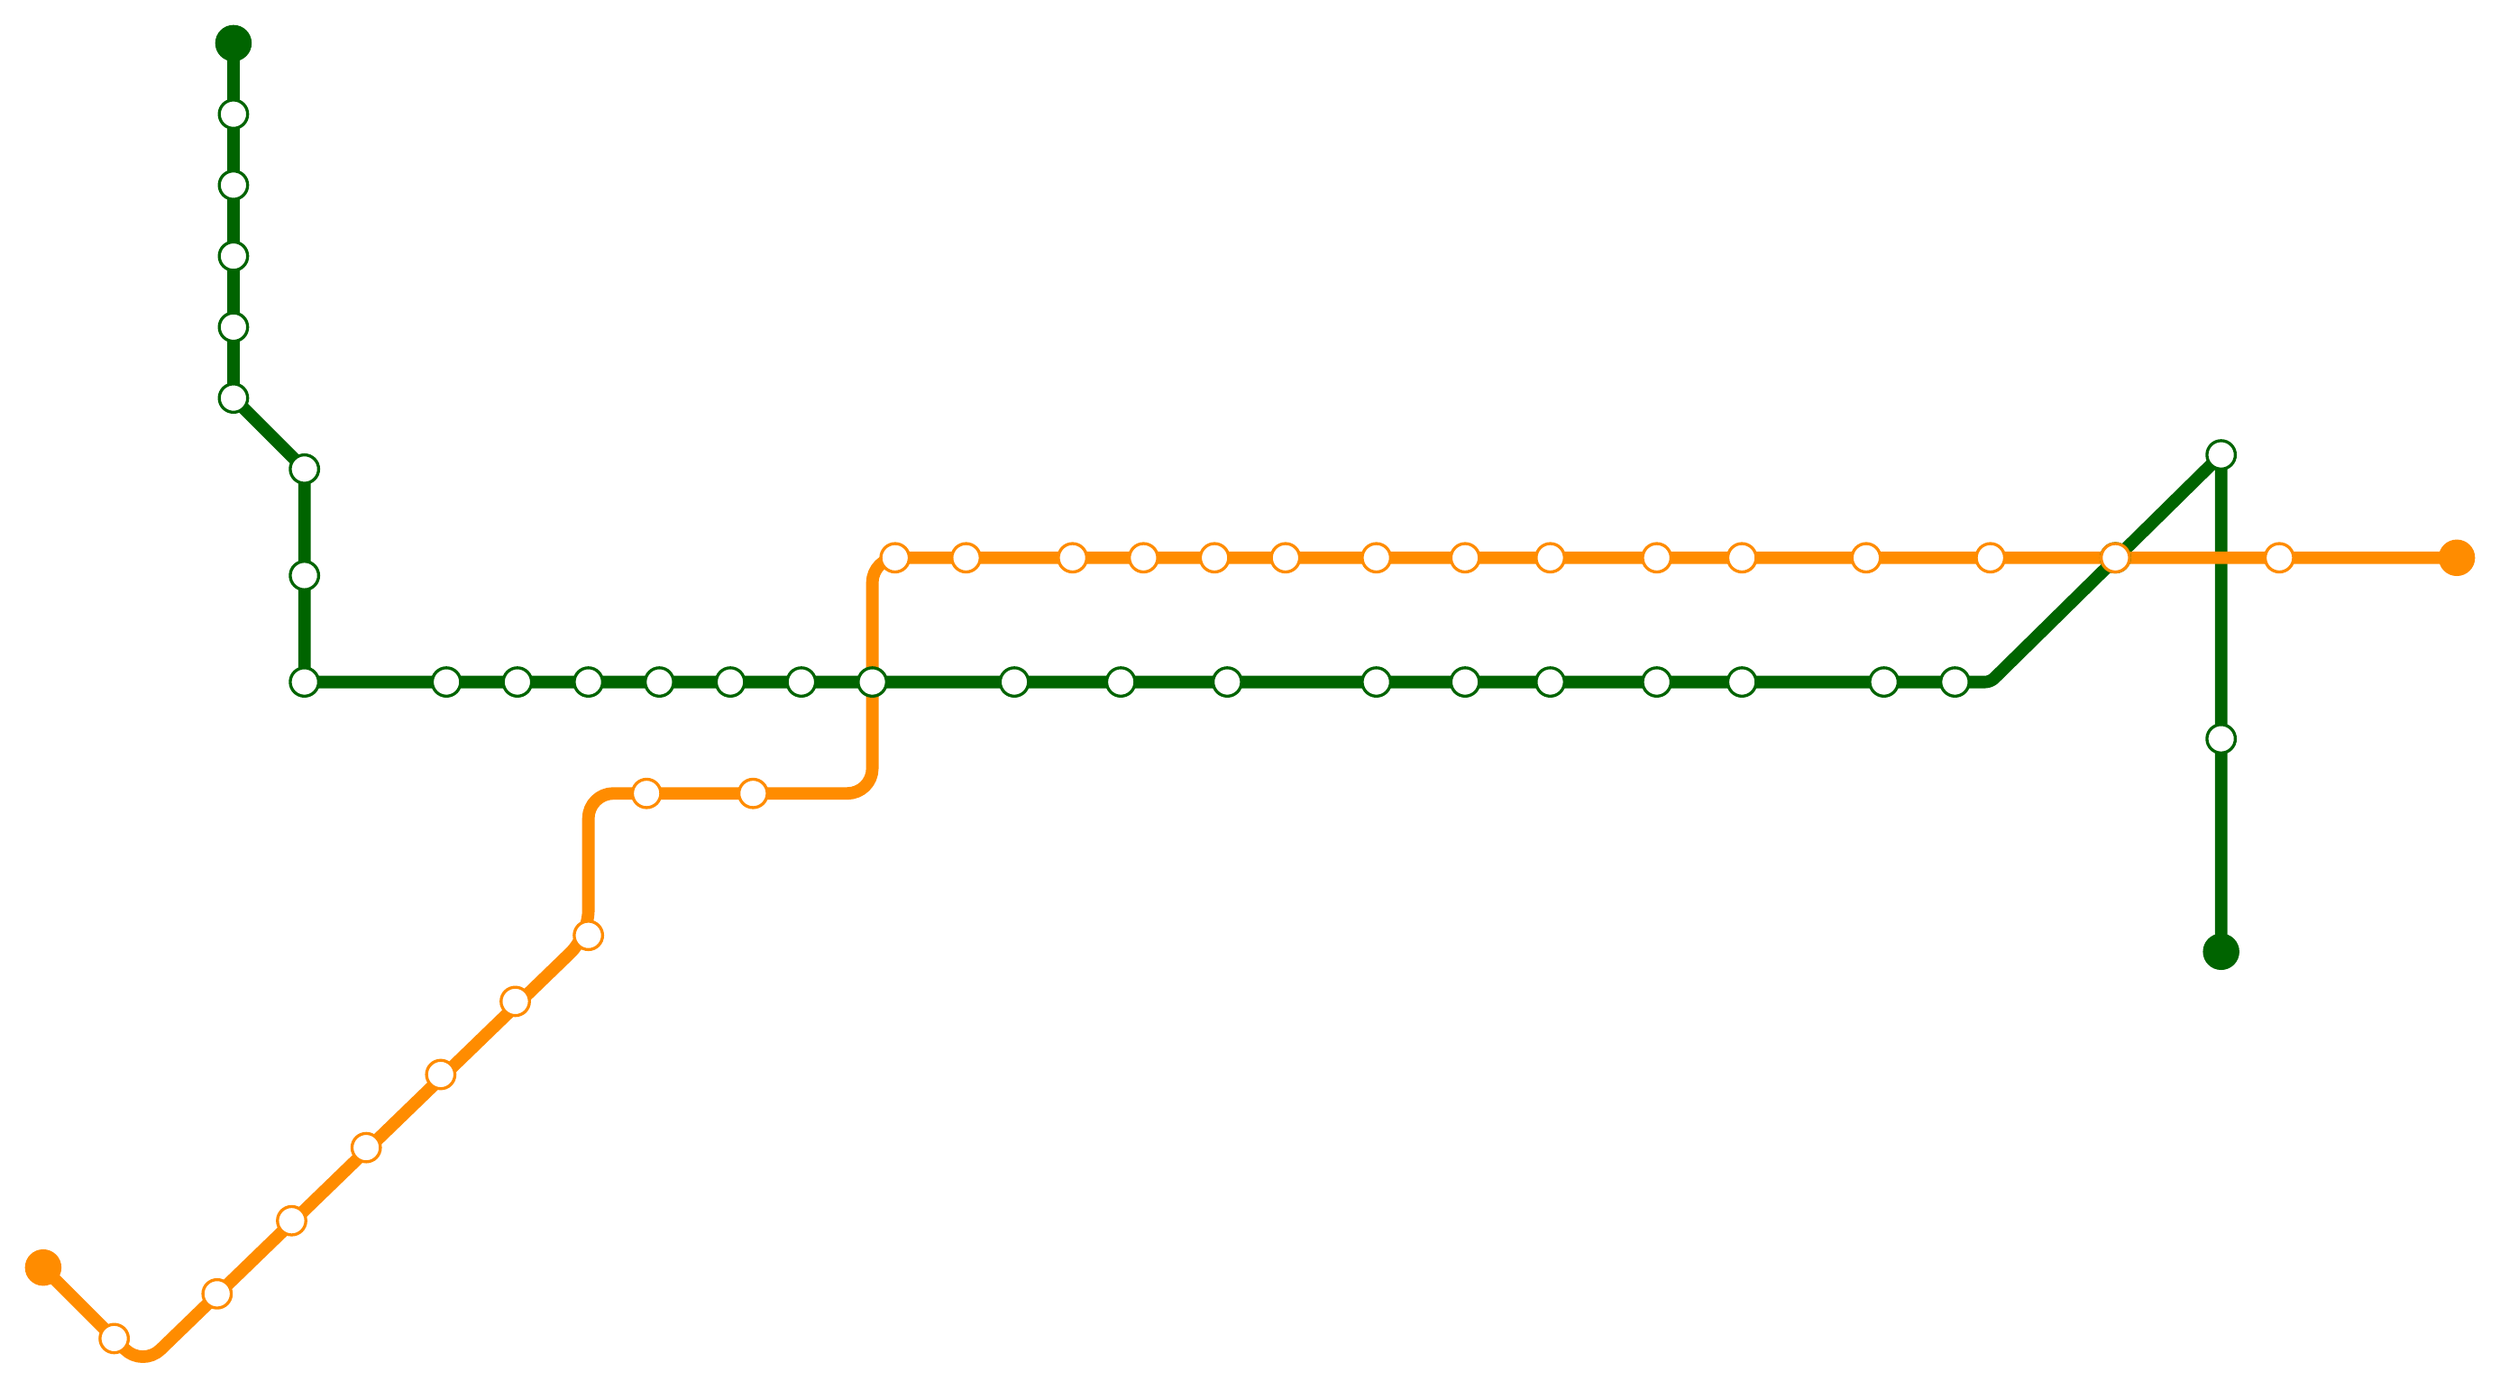
\begin{tikzpicture}[
stop1/.style={stop=DarkGreen},stop1-terminal/.style={stop-terminal=DarkGreen},
stop2/.style={stop=DarkOrange},stop2-terminal/.style={stop-terminal=DarkOrange}]

% 一号线
\begin{scope}
\begin{pgfonlayer}{line}
\draw [line=DarkGreen,rounded corners=2pt] (0,0) -- (0,-5) -- (1,-6) -- (1,-9) -- (3,-9) -- (24.75,-9) -- (28,-5.8) -- (28,-12.8);
\end{pgfonlayer}
\begin{pgfonlayer}{stop}
\node at (0,0) [stop1-terminal] {};
\foreach \i in {-1,-2,...,-5} {\node at (0,\i) [stop1] {};} 
\foreach \i in {-6,-7.5,-9} {\node at (1,\i) [stop1] {};} %宝安中心,新安,前海湾
\foreach \i in {3,4,...,9} {\node at (\i,-9) [stop1] {};} %世界之窗
\foreach \i in {11,12.5,14,16.1} {\node at (\i,-9) [stop1] {};} %车公庙
\foreach \i in {17.35,18.55,20.05,21.25,23.25,24.25} {\node at (\i,-9) [stop1] {};} %科学馆
\node at (26.51,-7.25) [stop1] {}; %大剧院
\node at (28,-5.8) [stop1] {}; %老街
\node at (28,-9.8) [stop1] {}; %国贸
\node at (28,-12.8) [stop1-terminal] {};
\end{pgfonlayer} 
\end{scope} 

% 二号线
\begin{scope}[shift={(-2.68,-17.25)}]
\begin{pgfonlayer}{line}
\draw [line=DarkOrange,rounded corners=10pt] (0,0) -- (1.4,-1.4) -- (7.68,4.68) -- (7.68,6.68)
-- (11.68,6.68) -- (11.68,10) -- (34,10);
\end{pgfonlayer}
\begin{pgfonlayer}{stop}
\node at (0,0) [stop2-terminal] {};
\node at (1,-1) [stop2] {};
\foreach \i in {1,2,...,5} {\node at (1.4+\i*1.05,-1.4+\i*1.03) [stop2] {};}
\node at (7.68,4.68) [stop2] {}; %后海
\node at (8.5,6.68) [stop2] {};
\node at (10,6.68) [stop2] {}; %世界之窗
\node at (12,10) [stop2] {}; %侨城北
\node at (13,10) [stop2] {}; %深康
\node at (14.5,10) [stop2] {};%安托山
\node at (15.5,10) [stop2] {};%侨香
\node at (16.5,10) [stop2] {}; %香蜜
\node at (17.5,10) [stop2] {}; %香梅北
\node at (18.78,10) [stop2] {}; %景田
\node at (20.03,10) [stop2] {}; %莲花西
\node at (21.23,10) [stop2] {}; %福田
\node at (22.73,10) [stop2] {}; %市民中心
\node at (23.93,10) [stop2] {}; %岗厦北
\node at (25.68,10) [stop2] {}; %华强北
\node at (27.43,10) [stop2] {}; %燕南
\node at (29.19,10) [stop2] {}; %大剧院
\node at (31.5,10) [stop2] {}; %湖贝
\node at (34,10) [stop2-terminal] {}; %新秀 
\end{pgfonlayer}
\end{scope}

\end{tikzpicture}
\end{document} 
